\documentclass[11pt]{article}
\usepackage[margin=1in]{geometry}
\usepackage{amsmath,amssymb}
\usepackage{lmodern}
\usepackage[T1]{fontenc}
\usepackage{enumitem}
\usepackage{microtype}
\usepackage{tikz}
\usetikzlibrary{arrows.meta,angles,quotes,calc,decorations.pathreplacing}

\title{2019A F=ma Exam Review}
\author{Nathan P.}
\date{January 12, 2026}

\begin{document}
\maketitle

\section*{Problem 3}
Use momentum conservation (essentially a perfectly inelastic collision).
Use energy conservation (no external forces) and consider convenient points: initial kinetic $=$ final kinetic of both (moving at the same speed) $+\,mgh$.
You can write $K$ as $p^2/2m$ to avoid doing $mv=(M+m)v'$, because momentum is conserved (it stays $mv$ for the system). $p$ is the total momentum and $m$ is the total mass, so
\[
K=\frac{(mv)^2}{2(M+m)}.
\]

\section*{Problem 4}
Problem-solving strategy: instead of thinking there's not enough info, what if you can solve for a ratio instead? $T\propto\sqrt{m/k}$. We have neither $m$ nor $k$, but we can easily find an expression for $m/k$ using basic energy conservation.
In SHM, velocity $=0$ implies an extreme. The equilibrium point is where $mg=kx$.
When you release it, at one point it passes the equilibrium point. If it travels $2x$, then the upward force is $2mg$ and the net force is $mg$ upward, which proves the top of the motion is the release point and the equilibrium point is halfway down. So $mg=kx$, $m/k=x/g$, and (subbing that in for $m/k$)
\[
T=2\pi\sqrt{\frac xg}.
\]

\section*{Problem 6}
Work in the frame of the plane. Rotating your coordinates shows that in the $y$ direction (perpendicular to the incline) the ball simply collides elastically (reversing $v_y$ when hitting the stationary plane) and bounces back to the same height (perpendicular distance from the incline), conserving the $y$-motion energy, while being accelerated in the $x$ direction by gravity.

\section*{Problem 8}
Pay attention to the fact that the problem states the earth has radius $R$ and the object is at a distance $R$ from the surface. So the $r$ in the circular orbit and escape $v$'s would be $2R$.
\[
v_c=\sqrt{\frac{GM}{r}},\qquad v_{\text{esc}}=\sqrt{\frac{2GM}{r}}.
\]
$\sqrt{2GM/3R}=\sqrt{4GM/3r}$ is between circular and escape, so it'll be in an elliptical orbit starting closest to earth.
(If $\sqrt{GM/r}>v>0$, then the object has an elliptical orbit starting furthest from earth.)

\section*{Problem 9}
Draw the vectors, do the math, and use the half-angle identity
\[
\sin\frac\theta2=\sqrt{\frac{1-\cos\theta}{2}}.
\]

\section*{Problem 10}
The question said ``if the remaining shape has mass $M$,'' which implies the full disk has more than $M$.
To avoid arithmetic errors, set the original to $m$ and leave the final as $M$, then convert from $M$ to $m$. Similarly, for other problems, feel free to create your own variables and convert at the end.

\section*{Problem 12}
This is a challenging math-related problem. Identify the goal; this is very important. Know clearly what you're trying to find: the time between bounces $\tau$ as a function of the total time $t$.
The total time is found via the sum of a finite geometric series:
\[
\frac{a(1-r^n)}{1-r}.
\]
You'll be able to solve for the time for the $n$th bounce, $\tau(n)=\tau\alpha^n$, in terms of $t$.
Combining the total time and the time for the $n$th bounce eliminates $n$, and you see the linear relationship between $\tau(n)$ and $t$.

\section*{Problem 14}
Coriolis acceleration $=-2\,\boldsymbol\omega\times\mathbf v$.
Use $d=\tfrac12at^2$ for the deflection and $x=vt$ for the distance travelled, both in the rotating frame.

\section*{Problem 15}
Period of rotation $=$ time in the air.
Since the rod is initially upright (vertical), the initial horizontal velocity is the standard tangential $v=r\omega$, where $r$ is the distance to the com.

\section*{Problem 18}
Key idea: work done by the launcher $=\Delta K$ for the wedge.
OR: initial potential stored in the launcher $=$ final $K$ of the wedge.
Whether you approach it with the work-energy theorem or energy conservation depends on what you include in your system.

\section*{Problem 19}
The easiest way is to compare the new to the old restoring force ($mg$) to get $g_{\text{eff}}=g/2$, and use $\omega=\sqrt{g_{\text{eff}}/L}$.

\section*{Problem 20}
Balance the torques. For stability, the restoring torque must be greater than the destabilizing torque.
$dx=L\,d\theta$.

\section*{Problem 24}
$F=-dU/dx$. Once you have the restoring force, you can get $\omega$ and $T$.
$T_{\min}$ is the shorter period of $x$ or $y$, which occurs if the particle only moves in that dimension (and isn't moving in the other).
$T_{\max}$ occurs when there's oscillation in both dimensions, and the period only resets once they synchronize again, so it must be $\operatorname{LCM}(T_x,T_y)$.
(The foundation is that the function $U(x,y)$ has no cross terms like $xy$, so we can treat the $x$ and $y$ directions independently.)

\section*{Problem 25}
Bernoulli: $\rho gh=\tfrac12\rho v^2$.
In the rotating frame when turning, there is a centrifugal acceleration $v^2/r$, so $g_{\text{eff}}$ is at an angle to the vertical. Therefore the water surface will tilt, and the ``effective'' height also isn't just $h$.
Geometry: $h_{\text{eff}}=h\cos\theta=h\,\dfrac{g}{g_{\text{eff}}}$, so
\[
v=\sqrt{2g_{\text{eff}}h_{\text{eff}}}=\sqrt{2gh}.
\]

\begin{center}
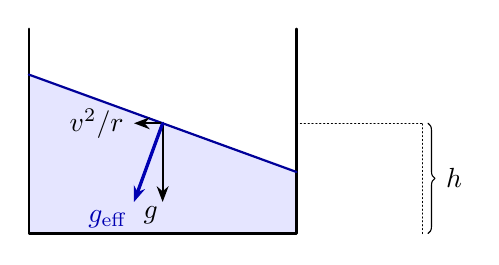
\begin{tikzpicture}[scale=1.0, line cap=round, line join=round, >={Stealth[length=2mm]}]
  % surface tilted by theta = 20 deg, perpendicular to g_eff
  \fill[blue!10] (0,0) -- (3.4,0) -- (3.4,{1.4-1.7*tan(20)}) -- (0,{1.4+1.7*tan(20)}) -- cycle;
  \draw[thick] (0,2.6) -- (0,0) -- (3.4,0) -- (3.4,2.6);
  \draw[thick, blue!60!black] (0,{1.4+1.7*tan(20)}) -- (3.4,{1.4-1.7*tan(20)});
  \coordinate (C) at (1.7,1.4);
  \draw[->, thick] (C) -- ++(0,-1.0) node[below left=-2pt] {$g$};
  \draw[->, thick] (C) -- ++({-tan(20)},0) node[left] {$v^2/r$};
  \draw[->, very thick, blue!70!black] (C) -- ++({-tan(20)},-1.0) node[below left=-1pt] {$g_{\text{eff}}$};
  \draw[densely dotted] (5.0,0) -- (5.0,1.4);
  \draw[decorate, decoration={brace, mirror, raise=2pt}] (5.0,0) -- (5.0,1.4) node[midway, right=5pt] {$h$};
  \draw[densely dotted] (3.4,1.4) -- (5.0,1.4);
\end{tikzpicture}
\end{center}

\end{document}
